\input{../header}
\usepackage{pgfplots}
\rhead{Your name: \rule{8cm}{0.15mm}}

\begin{document}

\section{Learning target IN1, version 1}

Use geometric formulas to find definite integrals.

\hrulefill

Here is the graph of a function $h(t)$, which is made up of only straight lines and parts of circles.

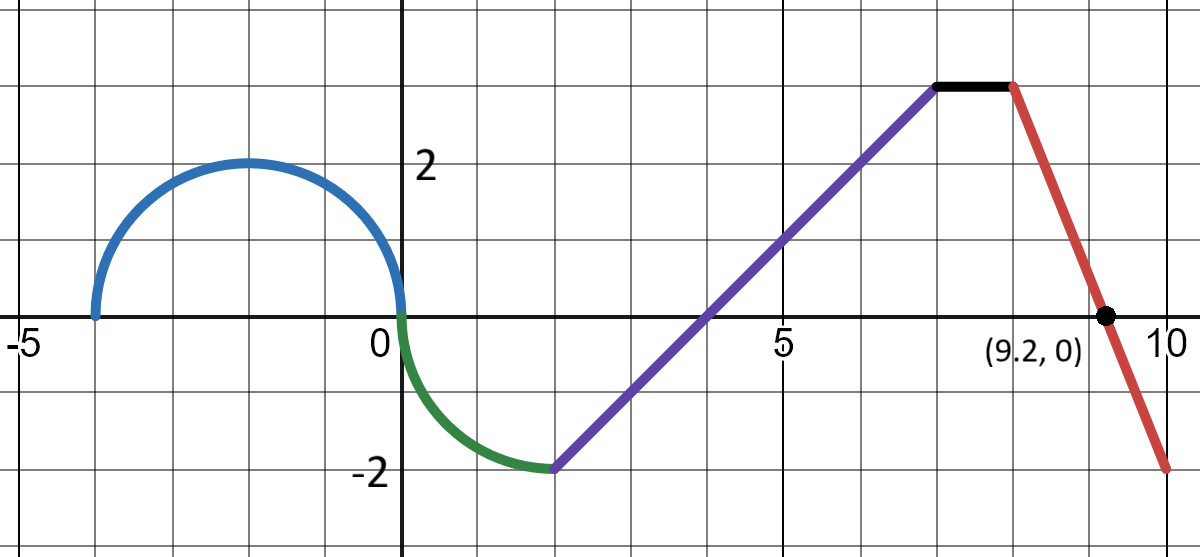
\includegraphics[width=\textwidth]{../images/IN1-v1.png}

Compute each of the following.

\begin{multicols*}{2}
{\everymath{\displaystyle}
\begin{enumerate}[(a)]
    \item $\int_{-4}^0 h(t)\, dt$

    \vfill
    \item $\int_0^2 h(t)\, dt$

    \vfill
    \item $\int_2^4 h(t)\, dt$

    \vfill
    \item $\int_4^7 h(t)\, dt$

    \vfill
    \columnbreak
    \item $\int_7^8 h(t)\, dt$

    \vfill
    \item $\int_8^{9.2} h(t)\, dt$

    \vfill
    \item $\int_{9.2}^{10} h(t)\, dt$

    \vfill
    \item $\int_{-4}^{10} h(t)\, dt$

\end{enumerate}
}
\end{multicols*}
%%%%%%%%%%%%%%%%%%%%%%%%%%%%%%%%%%%%%%%%%%%%%%%%%%%%%%%%%
\pagebreak
%%%%%%%%%%%%%%%%%%%%%%%%%%%%%%%%%%%%%%%%%%%%%%%%%%%%%%%%%

\section{Learning target IN1, version 2}

Use geometric formulas to find definite integrals.

\hrulefill

Here is the graph of a function $g(x)$, which is made up of only straight lines and parts of circles.

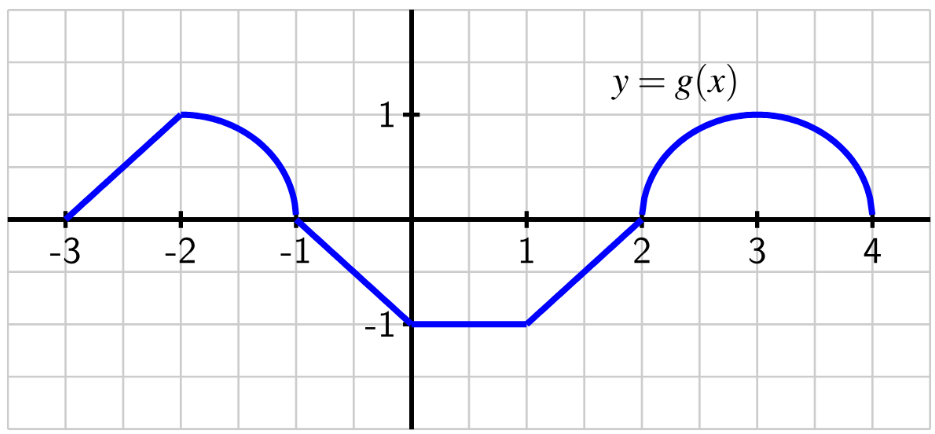
\includegraphics[width=\textwidth]{../images/IN1-v2.png}

Compute each of the following.

\begin{multicols*}{2}
{\everymath{\displaystyle}
\begin{enumerate}[(a)]
    \item $\int_{-3}^{-2} g(x)\ dx$

    \vfill
    \item $\int_{-2}^{-1} g(x)\ dx$

    \vfill
    \item $\int_{-1}^0 g(x)\ dx$

    \vfill
    \item $\int_0^1 g(x)\ dx$

    \vfill
    \columnbreak
    \item $\int_1^2 g(x)\ dx$

    \vfill
    \item $\int_2^4 g(x)\ dx$

    \vfill
    \item $\int_{-3}^4 g(x)\ dx$

    \vfill
    

\end{enumerate}
}
\end{multicols*}
%%%%%%%%%%%%%%%%%%%%%%%%%%%%%%%%%%%%%%%%%%%%%%%%%%%%%%%%%
\pagebreak


\section{Learning target IN1, version 3}

Use geometric formulas to find definite integrals.

\hrulefill

Here is the graph of a function $q(t)$, which is made up of only straight lines and parts of circles.

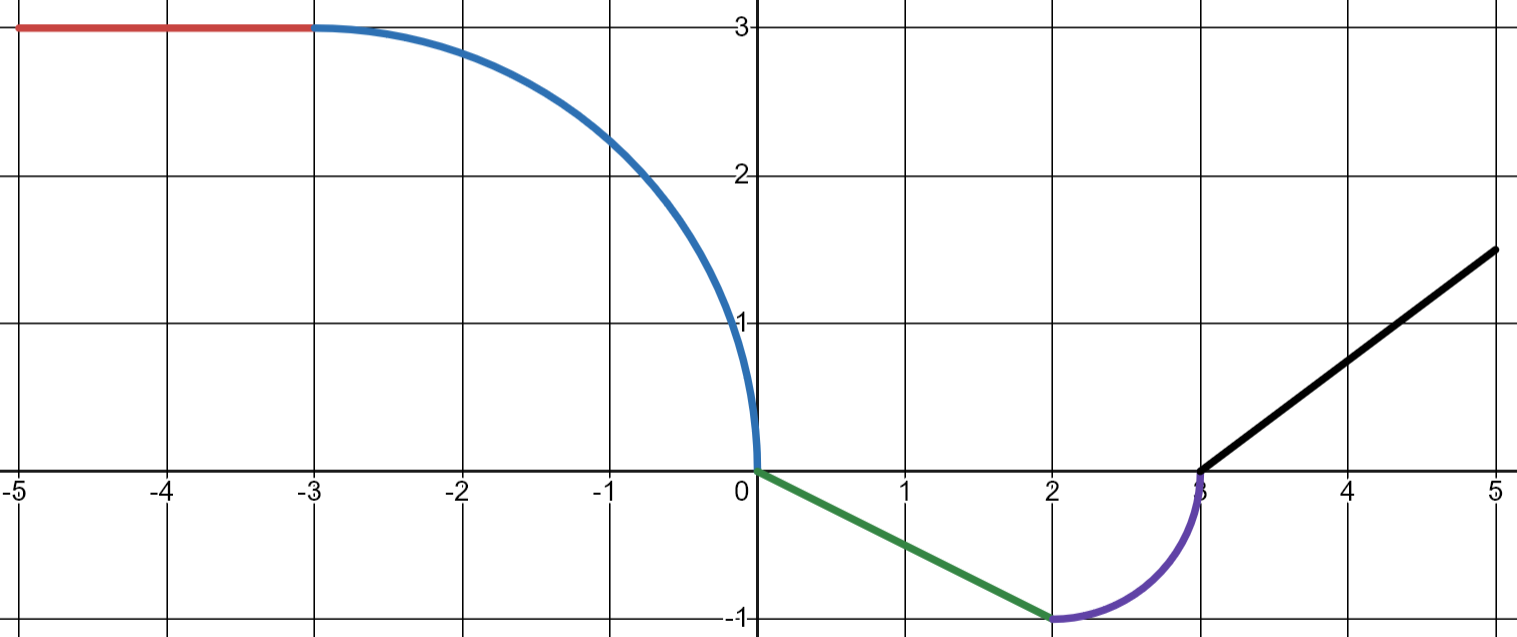
\includegraphics[width=\textwidth]{../images/IN1-v3.png}

Compute each of the following.

\begin{multicols*}{2}
{\everymath{\displaystyle}
\begin{enumerate}[(a)]
    \item $\int_{-5}^{-3} q(t)\ dt$

    \vfill
    \item $\int_{-3}^{0} q(t)\ dt$

    \vfill
    \item $\int_{0}^2 q(t)\ dt$

    \vfill
    \item $\int_2^3 q(t)\ dt$

    \vfill
    \columnbreak
    \item $\int_3^5 q(t)\ dt$

    \vfill
    \item $\int_{-3}^2 q(t)\ dt$

    \vfill
    \item $\int_{-5}^5 q(t)\ dt$

    \vfill
    

\end{enumerate}
}
\end{multicols*}
%%%%%%%%%%%%%%%%%%%%%%%%%%%%%%%%%%%%%%%%%%%%%%%%%%%%%%%%%
\pagebreak

\section{Learning target IN1, version 4}

Use geometric formulas to find definite integrals.

\hrulefill

Here is the graph of a function $N(t)$, which is made up of only straight lines and parts of circles.

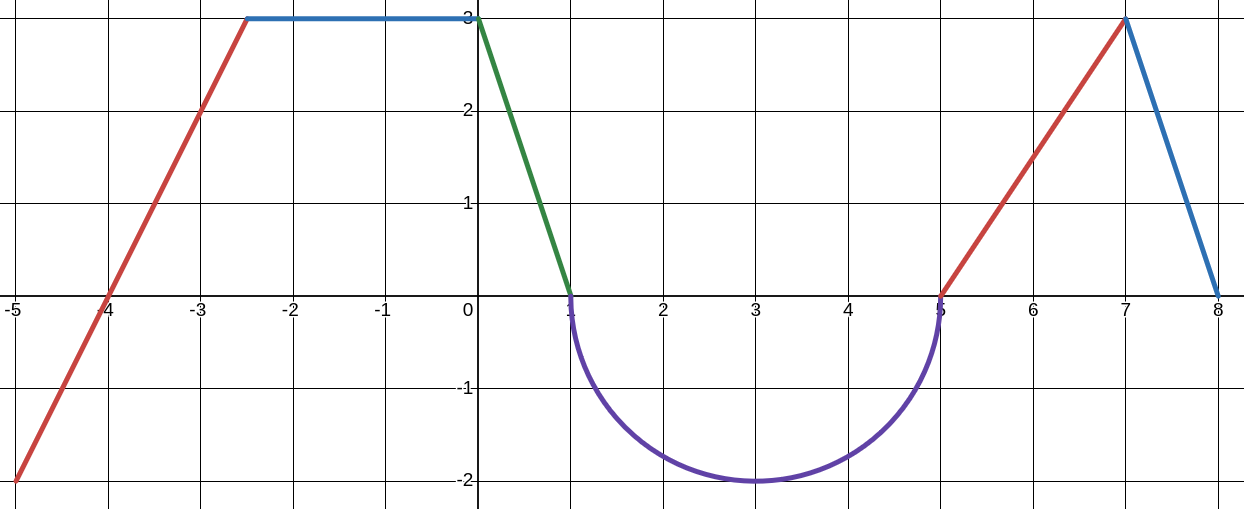
\includegraphics[width=\textwidth]{../images/IN1-v4.png}

Compute each of the following.

\begin{multicols*}{2}
{\everymath{\displaystyle}
\begin{enumerate}[(a)]
    \item $\int_{-5}^{-4} N(t)\ dt$

    \vfill
    \item $\int_{-4}^{-2.5} N(t)\ dt$

    \vfill
    \item $\int_{-2.5}^0 N(t)\ dt$

    \vfill
    \item $\int_0^1 N(t)\ dt$

    \vfill
    \columnbreak
    \item $\int_1^5 N(t)\ dt$

    \vfill
    \item $\int_{5}^7 N(t)\ dt$

    \vfill
    \item $\int_{7}^8 N(t)\ dt$

    \vfill
    \item $\int_{-5}^8 N(t)\ dt$
    

\end{enumerate}
}
\end{multicols*}
%%%%%%%%%%%%%%%%%%%%%%%%%%%%%%%%%%%%%%%%%%%%%%%%%%%%%%%%%
\pagebreak
%%%%%%%%%%%%%%%%%%%%%%%%%%%%%%%%%%%%%%%%%%%%%%%%%%%%%%%%%
\end{document}